\documentclass[10pt]{report}
\usepackage[utf8]{inputenc}
\usepackage[T1]{fontenc}
\usepackage{graphicx}
\usepackage[normalem]{ulem}
\usepackage{amsmath}
\usepackage{amssymb}
\usepackage{authblk}
\usepackage{minted}
\usepackage{titlepic}
\usepackage{booktabs}
% \title{$\vcenter{\hbox{
\includegraphics[width=\linewidth]{images/ADM.jpeg}}}$ \\ Progetto Basi di Dati}
% \author{Buglione Giuseppe}
% \author{Calcagno Mario}
% \author{Calculli Francesco}
% \titlepic{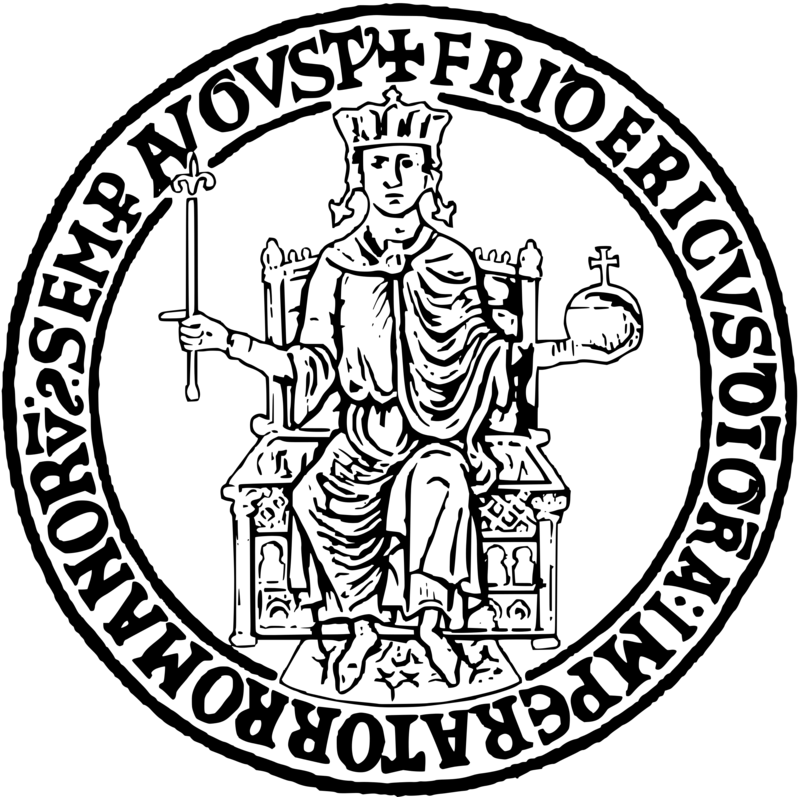
\includegraphics[width=\linewidth]{images/F2.png}} % F2.png
% \affil{Dipartimento delle Tecnologie dell'Informazione, Università Federico II}
% \date{a.a. 2024/2025}
\begin{document}
% \maketitle
\begin{titlepage}
  \centering
  
\includegraphics[width=0.75\linewidth]{images/ADM.jpeg}\par
  {\Large \textsc{\texttt{ASTRADM}}\par}
  {\Large\itshape Buglione Giuseppe\par}
  {\Large\itshape Calcagno Mario\par}
  {\Large\itshape Calculli Francesco\par}
  {\Large\itshape Dipartimento delle Tecnologie dell'Informazione, Università Federico II\par}
  \vfill
  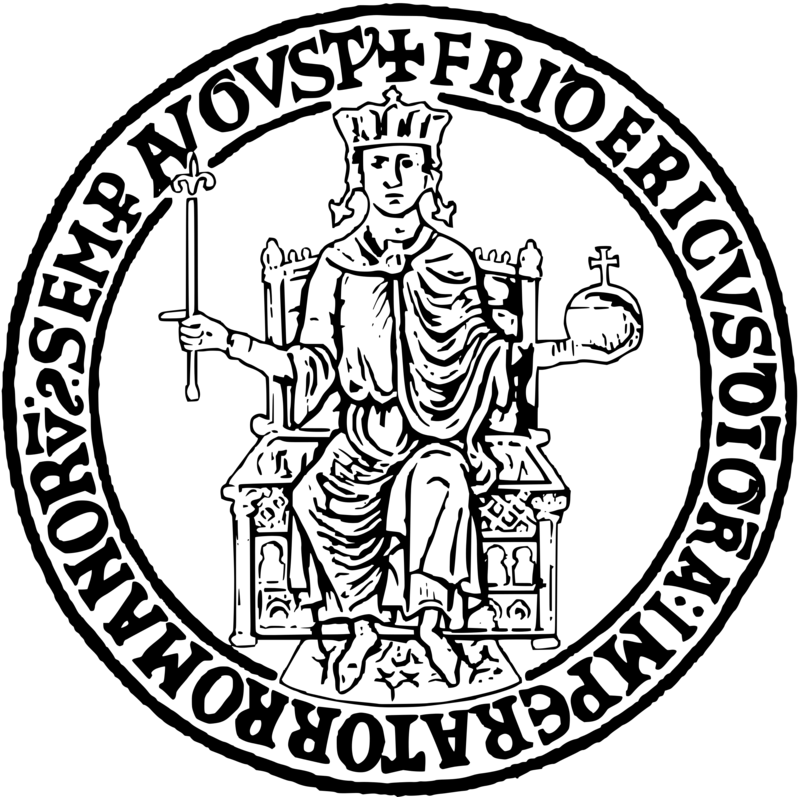
\includegraphics[width=0.15\linewidth]{images/F2.png}
\end{titlepage}

\tableofcontents
\chapter{Introduzione}
% DONE: scrivere introduzione
% DONE: scegliere nome del programma
% DONE: scirvere specifica funzionale
% DONE: scrivere specifica sugli utenti e policy di sicurezza
\texttt{ASTRODM} nasce con l'intento di fornire un sistema informatico
per l'analisi e la gestione dei dati raccolti durante le missioni
d'esplorazione spaziali.  Il sistema permette da parte dei membri
dell'equipaggio una gestione completa delle informazioni provenienti
dai sensori e fornire un monitoraggio dettagliato delle operazioni in
corso.


% DONE: scrivere specifica informale
% DONE: risolvere il problema del da capo
\section{Specifica Informale} 
A.D.M. (Astra Data Management), un sistema informatico ,a supporto per i membri delle future missioni di esplorazioni lunari

\subsection{Obiettivi Principali:}
\begin{itemize}
\item  La gestione e analisi dei dati raccolti da sensori sparsi sulla superficie lunare 
\item  Gestione delle possibili anomalie riscontrabili e dei conseguenti interventi di riparazione.
\item  Gestori di robot autonomi per operazioni sul campo.
\item  Coordinazione in tempo reale della attivita dei membri della missione
\item  Monitoraggio delle operazioni in corso e dei relativi report.
\end{itemize}

%%% Local Variables:
%%% mode: LaTeX
%%% TeX-master: "Tesina"
%%% End:

\section{Specifica sui dati}
Come visto già nella specifica informale, è necessario poter gestire i seguenti dati:
\begin{description}
\item[Anomalie] Possibili guasti o anomalie di un sensore
\item[Intervento] Interventi di riparazione, possono coinvolgere uno o più operatori
\item[Membri dell'equipaggio] Dati degli operatori assegnati ad una missione
\item[Missione] Missione di esplorazione lunare
\item[Report] Report sull'esito di una missione da parte di un operatore
\item[Rilevazione] Le rilevazioni fatte da un sensore
\item[Robot] Una delle risorse impiegate durante una missione
\item[Sensore] Una delle risorse impiegate durante una missione
\end{description}

%%% Local Variables:
%%% mode: LaTeX
%%% TeX-master: "Tesina"
%%% End:

\section{Specifica delle funzionalità}
La piattaforma deve mettere a disponibilità le seguenti funzionalità:
\begin{itemize}
  \item Monitoraggio delle operazioni
  \item Gestione dei sensori sulla superficie lunare
  \item Supporto a diverse operazioni di analisi statistica
\end{itemize}
In particolare gli operatori devono essere in grado di:
\begin{itemize}
  \item Registrare o cancellare le missioni
  \item Registrare o cancellare le anomalie
  \item Inserire i report
\end{itemize}

%%% Local Variables:
%%% mode: LaTeX
%%% TeX-master: "Tesina"
%%% End:

\section{Specifica utenti e policy di sicurezza}
Creato lo schema della basi di dati:
\mint{sql}/CREATE SCHEMA ASTRADM;/
\par
Si è deciso di creare i seguenti utenti:
\begin{description}
\item[Database Administrator] DBA, con controllo completo della base di dati
  \begin{minted}{sql}
    CREATE USER astradm_dba IDENTIFIED BY astradm_dba;
    GRANT DBA TO astradm_dba;
  \end{minted}
\item[Admin] Amministratore di sistema, ha i permessi CREATE, DROP, INSERT,UPDATE, DELETE e SELECT, oltre alla
  possibilità di creare nuove stored procedures
  \begin{minted}{sql}
    CREATE ROLE admin;
    GRANT CONNECT TO admin;
    GRANT RESOURCE TO admin;
  \end{minted}
  %TODO: Rivedere creazione ruolo operator
\item[Operatore] Un operatore ha i permessi INSERT, UPDATE, DELETE, SELECT.
  \begin{minted}{sql}
    CREATE ROLE operator;
    GRANT CONNECT TO operator;
    GRANT SELECT ON ASTRADM.* TO operator;
    GRANT INSERT,UPDATE, DELETE ON ASTRADM.* TO operator
  \end{minted}
\end{description}

%%% Local Variables:
%%% mode: LaTeX
%%% TeX-master: "Tesina"
%%% End:


%%% Local Variables:
%%% mode: LaTeX
%%% TeX-master: "Tesina"
%%% End:

\chapter{Progettazione Concettuale}
In questa sezione si affronta la traduzione delle problematiche presentate in un
modello \textbf{Entity-Relationship}, abbreviato in ``E/R'', definendo le entità
e le relazioni che lo compongono.
% TODO: scrivere discussione dello schema ER portante
% DONE: definire schema ER portante
\section{Schema E/R portante}
Analizzando le problematiche presentate si è arrivati all'individuazione delle
seguenti entità fondamentali:
\begin{description}
\item[Membro] Anagrafica dei membri dell'equipaggio
\item[Missione] Affidata dall'agenzia spaziale internazionale per l'esplorazione e analisi del
  terreno lunare
\item[Report] Report redatti dai membri sull'esito di una missione
\item[Robot] Una delle risorse utilizzabili in una missione
\item[Sensore] La risorsa principale utilizzata in una missione
\end{description}
\begin{figure}
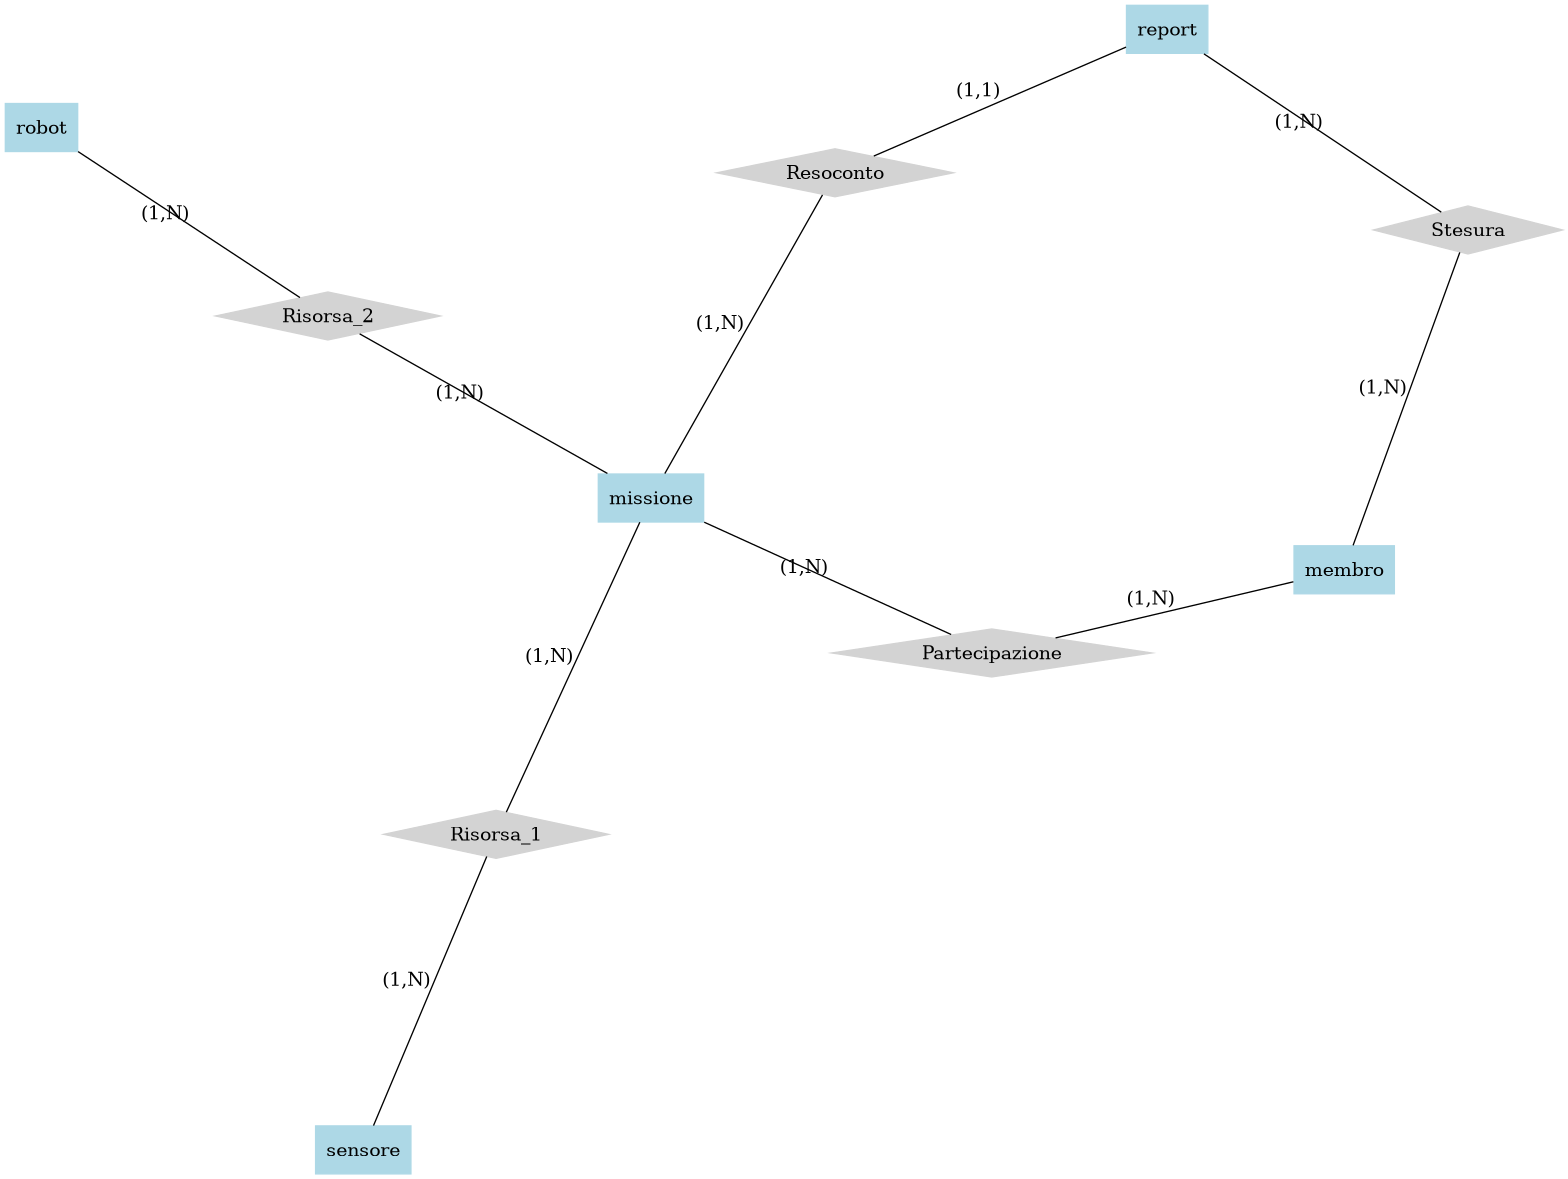
\includegraphics[width=\linewidth]{images/er-portante.png}
\caption{Modello E/R portante per \texttt{ASTRADM}}
\label{fig:er-portante}
\end{figure}           
Come visibile da \ref{fig:er-portante} sono state individuate le seguenti relazioni principali:
\begin{description}
\item[Partecipazione] Indica la partecipazione di un'\textbf{membro} ad una
  data \textbf{missione}
\item[Resoconto] Indica la \textbf{missione} a cui si riferisce un dato \textbf{report}
\item[\texttt{Risorsa\_1}] Indica l'utilizzo di una data risorsa di
  tipo \textbf{sensore} in una data \textbf{missione}
\item[\texttt{Risorsa\_2}] Indica l'utilizzo di una data risorsa di
  tipo \textbf{robot} in una data \textbf{missione}
\item[Stesura] Indica il \textbf{membro} autore di un dato \textbf{report}
\end{description}


% TODO: Scrivere discussione dello schema ER finale
\paragraph{Schema E/R finale}


%%% Local Variables:
%%% mode: LaTeX
%%% TeX-master: "Tesina"
%%% End:

\chapter{Progettazione Logica}
Di qui si tratta della progettazione logica del database per
\texttt{ASTRADM}

\section{Trasformazione del modello E/R}
Riferendoci al modello raffigurato in \ref{fig:er} possiamo cominciare
a discutera della semplificazione e della specializzazione del
modello. Partendo dal modello \ref{fig:er} possiamo vedere come gli attributi:
\begin{description}
\item[descrizione] dell'entità \textbf{Intervento}
\item[posizione] dell'entità \textbf{Sensore}
\end{description}
siano composti. Di conseguenza è possibili trasformarli nel seguente modo:
\begin{center}
  descrizione $\rightarrow$ sostituzione,riparazione, calibrazione
\end{center}
e
\begin{center}
  posizione $\rightarrow$ latitudine, longitudine, altitudine
\end{center}

Di conseguenza il modello diventa
\begin{figure}[ht]
  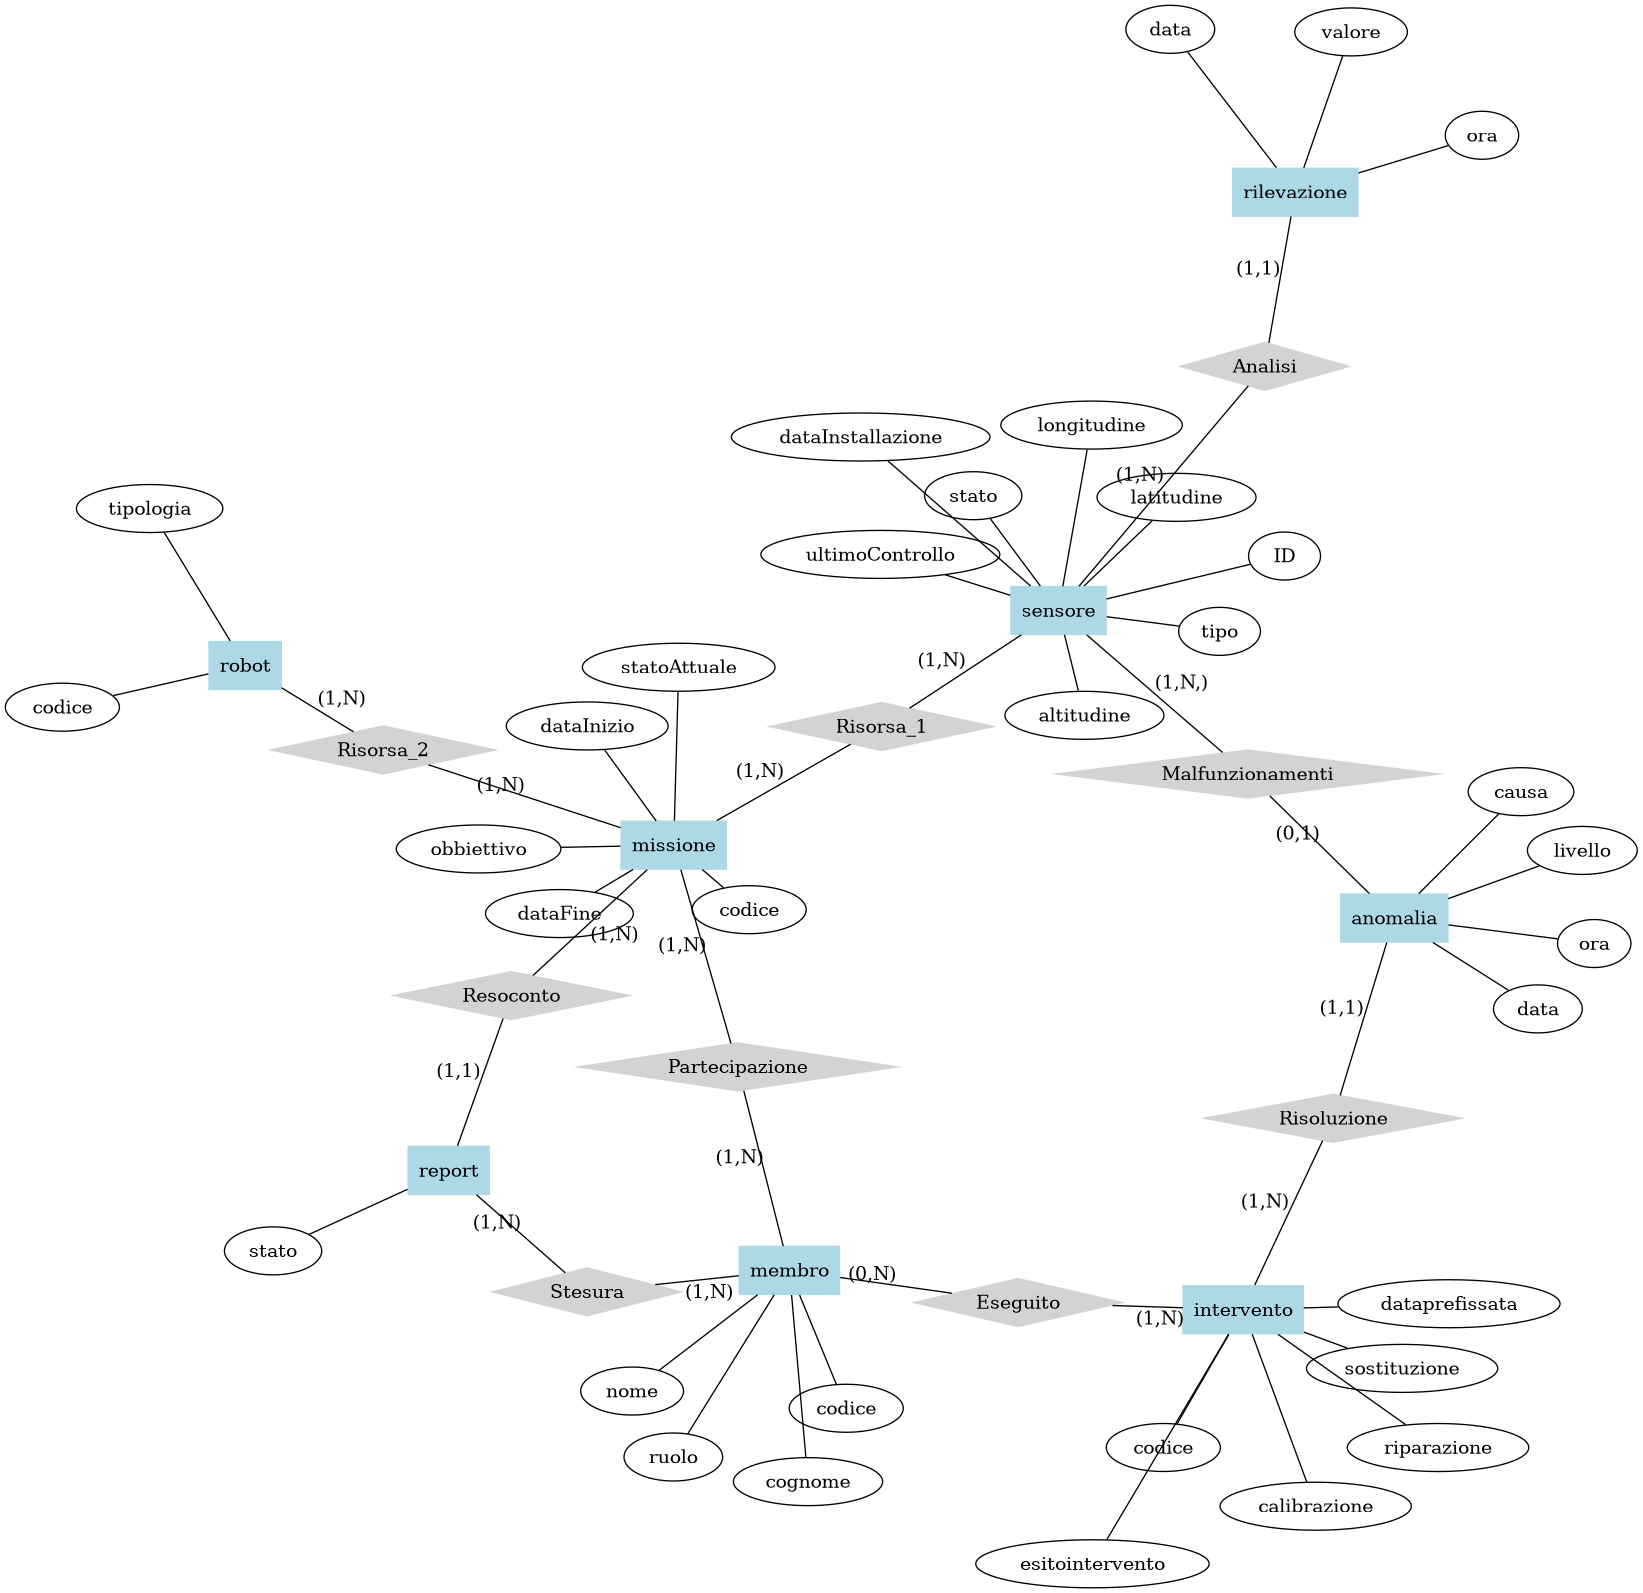
\includegraphics[width=\linewidth]{images/er-finale.png}
  \caption{Modello ER finale per \texttt{ASTRADM}}
  \label{fig:er-finale}
\end{figure}
 	
%%% Local Variables:
%%% mode: LaTeX
%%% TeX-master: "Tesina"
%%% End:

\section{Creazione Schema Relazionale}
In questa sezione ci occupiamo della creazione dello schema relazionale partendo dal
modello E/R in \ref{fig:er-finale}. Per la traduzione da modello E/R a schema relazionale
si seguono le seguenti regole:
\begin{enumerate}
\item Ciascuna \textit{entità} viene trasformata in una relazione,
  dove gli attributi dell'entità diventano gli attributi della
  relazione, con la chiave primaria dell'entità che diventa
  l'identificatore della relazione
\item Le relazioni vengono tradotte in base alla loro cardinalità:
\begin{description}
\item [uno a uno] si traducono aggiungendo alle relazioni che traducono le entità dal lato uno gli
    attributi delle associazioni e gli identificatori delle entità lato molti. Questi ultimi saranno soggetti
    ad un vincolo di integrità referenziale con il corrispondente attributo delle entità dal lato molti
\item [uno a molti] si traducono aggiungendo alla relazione che traduce una delle due entità gli attributi
    dell’associazione, oltre che il suo identificatore che sarà soggetto sia ad un vincolo di unicità
    che di integrità referenziale con il corrispondente attributo dell’altra entità.
\item [molti a molti] si traduce in un relazione con lo stesso nome avente come attributi, gli attributi dell'associazione  
  e gli indentificativi dell'entita coinvolte, dove quest'ultime vanno a costituire un vincolo di integrita referenziale con
  l'attributo corrispondente dell'entità.
  \end{description}
\end{enumerate}

% TODO: Creare schema relazionale
Seguendo queste regole si ottiene il seguente schema:
\begin{itemize}
% TODO: Completare ANOMALIE
\item \texttt{ANOMALIE}(\underline{data}, \underline{ora}, causa, livello,SENSORI: sensorie,};
% TODO: Completare INTERVENTI
\item \texttt{INTERVENTI}(\underline{codice}, esito, calibrazione, riparazione, sostituzione, dataPrefissata);
% TODO: Completare MEMBRI
\item \texttt{MEMBRI}(\underline{codice}, nome, cognome, ruolo);
% TODO: Completare MISSIONI
\item \texttt{MISSIONI}(\underline{codice}, dataFine, obbiettivo, dataInizio, statoAttuale,REPORT:resoconto);
% TODO: Aggiungere Risorsa_1
\item \texttt{RISORSA_1}(\underline{SENSORI:sensore},\underline{MISSIONI:missione});
% TODO: Completare REPORT
\item \texttt{REPORT}(\underline{stato}, MEMBRI:autore);
% TODO: Completare RIVELAZIONI
\item \texttt{RILEVAZIONI}(\underline{data}, \underline{ora}, valore, SENSORI: sensore);
% TODO: Completare ROBOT
\item \texttt{ROBOT}(\underline{codice}, tipologia);
% TODO: Aggiungere Risorsa_2
\item \texttt{RISORSA_2}(\underline{Robot:robot},\underline{MISSIONI:missione});
% TODO: Completare SENSORI
\item \texttt{SENSORI}(\underline{ID}, stato, dataInstallazione, tipo, ultimoControllo, latitudine, altitudine, longitudine);
\end{itemize}

%%% Local Variables:
%%% mode: LaTeX
%%% TeX-master: "Tesina"
%%% End:


%%% Local Variables:
%%% mode: LaTeX
%%% TeX-master: "Tesina"
%%% End:

\chapter{Progettazione Fisica}
\section{Dimensionamento dei dati}
% TODO:Completare inserendo in numero di tuple
Per andare fare una stima sul volume che adranno ad occupare i vari dati in base allla loro tipologia, ci baseremo su:
\begin{itemize}
\item Tabelle/Schemi ottenute in fase di progettazione logica (sezione 3.2)
\item Il numero di missioni previste dall'agenzia spaziale
\end{itemize}
\subsection{Anomalia}
\begin{tabular}{|c|c|c|}
  \hline
  \multicolumn{3}{|c|}{\textbf{ANOMALIA}}\\
  \hline
  Attributo & Tipo & Spazio[BYTE] \\
  \hline
  data & DATE & 7 \\
  ora & DATE & 7 \\
  causa & VARCHAR(30) & 30 \\
  livello & INTEGGER & 4 \\
  sensore & INTEGER & 4 \\
  \hline
\end{tabular}
\begin{equation}
  \begin{aligned}
    D_{\text{anomalia}}&=(D_{\text{data}} + D_{\text{ora}} +D_{\text{causa}} +D_{\text{livello}} + D_{\text{sensore}}) \cdot N_{\text{anomalie}}=\\
    &=(7+7+30+4+4)\cdot x\cdot 10^6=x\cdot 49.6  \text{\textbf{MB}}\\
  \end{aligned}
\end{equation}
\subsection{Interventi}
\begin{tabular}{ |c|c|c|}
  \hline
  \multicolumn{3}{|c|}{\textbf{INTERVENTI}} \\
  \hline
  Atributo & Tipo & Spazio[BYTE] \\
  \hline
  codice & INTEGER & 4 \\
  esito & VARCHAR(20) & 20 \\
  calibrazione & VARCHAR(20) & 20 \\
  riparazione & VARCHAR(20) & 20 \\
  sostituzione & VARCHAR(20) & 20 \\
  dataPrefissata & DATE & 7 \\
  \hline
\end{tabular}
\begin{equation}
  \begin{aligned}
    D_{\text{interventi}} &=\\
    &=(D_{\text{codice}} + D_{\text{esito}} +D_{\text{calibrazione}} +D_{\text{riparazione}} + D_{\text{sostituzione}} + D_{text{dataPrefissata}}) \cdot  Nint =\\
    &=(4+20+20+20+20+7)\cdot x\cdot 10^6= \textbf{MB}
  \end{aligned}
\end{equation}
\subsection{Membri}
\begin{tabular}{ |c|c|c|}
  \hline
  \multicolumn{3}{|c|}{\textbf{MEMBRI}}\\
  \hline
  Atributo & Tipo & Spazio[BYTE] \\
  \hline
  codice & INTEGER & 4 \\
  nome & VARCHAR(30) & 30 \\
  cognome & VARCHAR(30) & 30 \\
  ruolo & VARCHAR(30) & 30\\
  \hline
\end{tabular}
\begin{equation}
  \begin{aligned}
    D_{\text{membri}} &=\\
    &=(D_{\text{codice}} + D_{\text{nome}} +D_{\text{cognome}} +D_{\text{ruolo}}) \cdot  N_{\text{membri}} =\\
    &=(4+30+30+30) \cdot x\cdot 10^6= \textbf{MB}
  \end{aligned}
\end{equation}
\subsection{Missioni}
\begin{tabular}{ |c|c|c|}
  \hline
  \multicolumn{3}{|c|}{\textbf{MISSIONI}}\\
  \hline
  Atributo & Tipo & Spazio[BYTE] \\
  \hline
  codice & INTEGER & 4 \\
  dataFine & DATE & 7 \\
  obbiettivo & VARCHAR(100) & 100 \\
  dataInizio & DATE & 7 \\
  statoAttuale  & VARCHAR(30) & 30 \\
  dataFine & VARCHAR(30) & 30 \\
  \hline
\end{tabular}
\begin{equation}
  \begin{aligned}
    &D_{\text{missioni}} =\\
    &=(D_{\text{codice}}+D_{\text{dataFine}}+D_{\text{obbietivo}}+D_{\text{dataInizio}}+D_{\text{statoA}}+D_{\text{dataFine}})\cdot N_{\text{miss}}=\\
    &=(4+7+100+7+30+30)\cdot x\cdot 10^6= \textbf{MB}
  \end{aligned}
\end{equation}
\subsection{Report}
\begin{tabular}{|c|c|c|}
  \hline
  \multicolumn{3}{|c|}{\textbf{REPORT}}\\
  \hline
  Atributo & Tipo & Spazio[BYTE] \\
  \hline
  stato & VARCHAR(30) & 30 \\
  autore & VARCHAR(30) & 30\\
  \hline
\end{tabular}

\begin{equation}
  \begin{aligned}
    D_{\text{report}} &=\\
    &=(D_{\text{stato}}+D_{\text{autore}})\cdot N_{\text{report}}=\\
    &=(30+30)\cdot x\cdot 10^6= \textbf{MB}
  \end{aligned}
\end{equation}
\subsection{Rilevazioni}
\begin{tabular}{|c|c|c|}
  \hline
  \multicolumn{3}{|c|}{\textbf{RILEVAZIONI}}\\
  \hline
  Atributo & Tipo & Spazio[BYTE] \\
  \hline
  data & DATE & 7 \\
  ora & DATE &  7 \\
  valore & INTEGER & 4 \\
  sensore & INTEGER & 4 \\
  \hline
\end{tabular}
\begin{equation}
  \begin{aligned}
    D_{\text{rivelazione}} &=\\
    &=(D_{\text{data}}+D_{\text{ora}}+D_{\text{valore}}+D_{\text{sensore}})\cdot N_{\text{rivelazione}}=\\
    &=(7+7+4+4+)\cdot x\cdot 10^6= \textbf{MB}
  \end{aligned}
\end{equation}
\subsection{Robot}
\begin{tabular}{ |c|c|c|}
  \hline
  \multicolumn{3}{|c|}{\textbf{ROBOT}}\\
  \hline
  Atributo & Tipo & Spazio[BYTE] \\
  \hline
  codice & INTEGER & 4\\
  tipologia & VARCHAR(30) & 30\\
  \hline
\end{tabular}
\begin{equation}
  \begin{aligned}
    D_{\text{robot}} &=\\
    &=(D_{\text{codice}}+D_{\text{tipologia}})\cdot N_{\text{robot}}=\\
    &=(4+30)\cdot x\cdot 10^6= \textbf{MB}
  \end{aligned}
\end{equation}
\subsection{Sensori}
\begin{tabular}{ |c|c|c|}
  \hline
  \multicolumn{3}{|c|}{\textbf{SENSORI}}\\
  \hline
  Atributo & Tipo & Spazio[BYTE] \\
  \hline
  ID & INTEGER & 4 \\
  stato & VARCHAR(30) & 30\\
  dataInstallazione & DATE & 7\\
  tipo & VARCHAR(30) & 30\\
  ultimoControllo & DATE & 7\\
  latitudine & DECIMAL(10,4) & 9\\
  altitudine & DECIMAL(10,4) & 9\\
  longitudine & DECIMAL(10,4) & 9\\
  \hline
\end{tabular}
\begin{equation}
  \begin{aligned}
    D_{\text{sensore}} &=\\
    &=(D_{\text{id}}+D_{\text{stato}}+D_{\text{dataInst}}+D_{\text{ultCont}}+D_{\text{lat}}+D_{\text{alt}}+D_{\text{long}})\cdot N_{\text{sen}}=\\
    &=(4+30+7+30+7+9+9+9)\cdot x\cdot 10^6= \textbf{MB}
  \end{aligned}
\end{equation}
\subsection{Gestione dello spazio e dell'affidabilità}
Dalle stime fatte precedentemente possiamo stimare un volume di informazioni pari:
\begin{equation}
  D_{\text{tot}}=X\\
\end{equation}

\section{Creazione del database}
%DONE: Da completare
Delineato il modello logico, tramite i comandi DDL possiamo inserire all'interno del data base gli schemi di relazioni associate alle tabelle.
\begin{description}

\subsection{Sensori}
\begin{minted}{sql}
CREATE SEQUENCE sensori_id_seq START WITH 1;
CREATE TABLE SENSORI (
    ID INTEGER DEFAULT sensori_id_seq.nextval NOT NULL,
    STATO VARCHAR(30) NOT NULL,
    DATAINSTALLAZIONE DATE NOT NULL,
    TIPO VARCHAR(30) NOT NULL,
    UTLIMOCONTROLLO DATE,
    LATITUDINE DECIMAL(10,4) NOT NULL,
    LONGITUDINE DECIMAL(10,4) NOT NULL,
    ALTITUDINE DECIMAL(10,4) NOT NULL,
    CONSTRAINT PK_ID PRIMARY KEY(ID)
);
\end{minted}

\subsection{Anomalie}
\begin{minted}{sql}
CREATE TABLE ANOMALIE(
    DATA DATE NOT NULL,
    ORA VARCHAR(8) NOT NULL,
    CAUSA VARCHAR(30) NOT NULL,
    LIVELLO INTEGER NOT NULL,
    SENSORE INTEGER NOT NULL,
    CONSTRAINT PK_ANOMALIE PRIMARY KEY (DATA,ORA),
     
     CONSTRAINT FK_ANOMALIE_SENSORI FOREIGN KEY
     ->(SENSORE) REFERENCES SENSORI (ID) ON DELETE CASCADE
);
\end{minted}

\subsection{Interventi}
\begin{minted}[breaklines]{sql}
CREATE SEQUENCE interventi_codice_seq START WITH 1;
CREATE TABLE INTERVENTI(
    CODICE INTEGER DEFAULT interventi_codice_seq.nextval NOT NULL,
    ESITO VARCHAR(20) NOT NULL,
    CALIBRAZIONE VARCHAR(20) NOT NULL,
    RIPARAZIONE VARCHAR(20) NOT NULL,
    SOSTITUZIONE VARCHAR(20) NOT NULL,
    DATAPREFISSATA DATE NOT NULL,
    CONSTRAINT PK_INTERVENTI PRIMARY KEY(CODICE)
);
\end{minted}

\subsection{Membri}
\begin{minted}[breaklines]{sql}
CREATE SEQUENCE membri_codice_seq START WITH 1;
CREATE TABLE MEMBRI(
    CODICE INTEGER DEFAULT membri_codice_seq.nextval NOT NULL,
    NOME VARCHAR(20) NOT NULL,
    COGNOME VARCHAR(20) NOT NULL,
    RUOLO VARCHAR(20) NOT NULL,
    CONSTRAINT PK_MEMBRI PRIMARY KEY(CODICE)
);
\end{minted}

\subsection{Report}
\begin{minted}[breaklines]{sql}
CREATE TABLE REPORT(
    STATO VARCHAR(30) NOT NULL,
    AUTORE INTEGER NOT NULL,
    CONSTRAINT PK_REPORT PRIMARY KEY(STATO),
    CONSTRAINT FK_REPORT_MEMBRI FOREIGN KEY(AUTORE)
    ->REFERENCES MEMBRI(CODICE) ON DELETE CASCADE
);
\end{minted}

\subsection{Missioni}
\begin{minted}[breaklines]{sql}
CREATE SEQUENCE missioni_codice_seq START WITH 1;
CREATE TABLE MISSIONI(
    CODICE INTEGER DEFAULT missioni_codice_seq.nextval NOT NULL,
    DATAFINE DATE NOT NULL,
    OBBIETTIVO VARCHAR(100) NOT NULL,
    DATAINIZIO DATE NOT NULL,
    STATOATTUALE VARCHAR(30) NOT NULL,
    RESOCONTO VARCHAR(30) NOT NULL,
    CONSTRAINT PK_MISSIONI PRIMARY KEY (CODICE),
    CONSTRAINT FK_MISSIONI_REPORT FOREIGN KEY
    ->(RESOCONTO) REFERENCES REPORT(STATO) ON DELETE CASCADE
);
\end{minted}

\subsection{Rilevazioni}
\begin{minted}[breaklines]{sql}
CREATE TABLE RILEVAZIONI(
    DATA DATE NOT NULL,
    ORA VARCHAR(8) NOT NULL, 
    VALORE INTEGER NOT NULL,
    SENSORE INTEGER NOT NULL,
    CONSTRAINT PK_RILEVAZIONI PRIMARY KEY(DATA,ORA),
    CONSTRAINT FK_RILEVAZIONI_SENSORI FOREIGN KEY(SENSORE)
    ->REFERENCES SENSORI (ID) ON DELETE CASCADE
    );
\end{minted}

\subsection{Robot}
\begin{minted}[breaklines]{sql}
CREATE SEQUENCE robo_codice_seq START WITH 1;
CREATE TABLE ROBOT(
    CODICE INTEGER DEFAULT robot_codice_seq.nextval NOT NULL,
    TIPOLOGIA VARCHAR(30),
    CONSTRAINT PK_ROBOT PRIMARY KEY(CODICE)
);
\end{minted}

\subsection{Risorsa\textsubscript{1}}
\begin{minted}[breaklines]{sql}
CREATE TABLE RISORSA_1(
    ROBOT INTEGER NOT NULL,
    MISSIONE INTEGER NOT NULL,
    CONSTRAINT PK_RISORSA_1 PRIMARY KEY(ROBOT,MISSIONE),

    CONSTRAINT FK_RISORSA1_ROBOT FOREIGN KEY(ROBOT)
    ->REFERENCES ROBOT(CODICE) ON DELETE CASCADE,
    
    CONSTRAINT FK_RISORSA1_MISSIONE FOREIGN KEY(MISSIONE) 
    ->REFERENCES MISSIONI(CODICE) ON DELETE CASCADE
    );
\end{minted}

\subsection{Risorsa\textsubscript{2}}
\begin{minted}[breaklines]{sql}
CREATE TABLE RISORSA_2(
    SENSORE INTEGER NOT NULL,
    MISSIONE INTEGER NOT NULL,
    CONSTRAINT PK_RISORSA_2 PRIMARY KEY (SENSORE,MISSIONE),
     
      CONSTRAINT FK_RISORSA2_SENSORE FOREIGN KEY(SENSORE)
   ->REFERENCES SENSORI(ID) ON DELETE CASCADE,

      CONSTRAINT FK_RISORSA2_MISSIONE FOREIGN KEY(MISSIONE)
     ->REFERENCES MISSIONI(CODICE) ON DELETE CASCADE,
    );
\end{minted}
\end{description}


%%% Local Variables:
%%% mode: LaTeX
%%% TeX-master: "Tesina"
%%% End:

%TODO: fare Dimensionamento dei dati
%TODO: fare Creazione del database
%TODO: fare Gestione degli indici
%TODO: fare Popolamento della base di dati

\chapter{Operazioni}
Per l'implementazione di funzionalità che la base dati deve offrire agli utento aviene mediante l'utilizzo di:
\begin{itemize}
\item Viste, sono delle tabelle, che vengono descritte in termini di altre tabelle, una \textbf{relazione virtuale}, dove sue tuple non sono memorizzate nella base dati ma ricavabili medianti interrogazioni, deliniando un iterfaccia messa a disposizione di utenti e applicazioni. La sua utilita si trova nei casi in cui si debbano vare tabelle che mettono in relazione campi di tabelle “distanti” nel modello logico.
\item Query, per verificare il corretto funzionamento della base di dati.
\item Trigger, sono procedure che si attivano quando vengono eseguite ogni volta che si fa un operazione stabilitasu un oggetto specifico della base dati.
\end{itemize}
\section{Viste}
\subsection{Vista dei sensori attivi con ultima rilevazione}
Creare una vista che unisca le informazioni sui sensori attivi con la loro ultima rilevazione registrata.
\begin{minted}{sql}
CREATE VIEW SENSORI_ATTIVI_RILEVAZIONI AS
SELECT SENSORI.ID AS SENSORI, RILEVAZIONI.DATA AS ULTIME_RILEVAZIONI
FROM SENSORI JOIN RILEVAZIONI ON SENSORI.ID = RILEVAZIONI.SENSORE
WHERE SENSORI.STATO='Attivo' AND RILEVAZIONI.DATA = (
    SELECT MAX(RILEVAZIONI.DATA)
    FROM RILEVAZIONI
    WHERE SENSORI.ID=RILEVAZIONI.SENSORE
);
\end{minted}
\subsection{Vista degli interventi completati e il loro esito}
Mostrare tutti gli interventi completati con dettagli su calibrazione, riparazione e sostituzione.
\begin{minted}[breaklines]{sql}
CREATE VIEW INTERVENTI-COMPLETATI AS
SELECT INTERVENTI.CODICE AS INTERVENTI,INTERVENTI.ESITO,INTERVENTI.CALIBRAZIONE,
->INTERVENTI.RIPARAZIONE,INTERVENTI.SOSTITUZIONE
FROM INTERVENTI
WHERE INTERVENTI.ESITO = 'Completato';
\end{minted}
\subsection{Vista dei membri e dei report creati}
Unire la tabella MEMBRI con REPORT per ottenere un elenco dei membri che hanno scritto report e il loro stato.
\begin{minted}{sql}
CREATE VIEW MEMBR_REPORT AS
SELECT MEMBRI.CODICE AS MEMBRO_CODE, REPORT.STATO AS STATO_REPORT
FROM MEMBRI JOIN REPORT ON MEMBRI.CODICE = REPORT.AUTORE;
\end{minted}
\subsection{Vista delle missioni con i robot assegnati}
Creare una vista che visualizzi le missioni attive e i robot assegnati tramite RISORSA\_1.
\begin{minted}{sql}
CREATE VIEW MISSIONI-ROBOT AS
SELECT MISSIONI.CODICE AS MISSIONI, RISORSA_1.ROBOT
FROM MISSIONI JOIN RISORSA_1 ON MISSIONI.CODICE = RISORSA_1.MISSIONE
WHERE MISSIONI.STATOATTUALE = 'Attiva'; 
\end{minted}
\subsection{Vista delle anomalie recenti}
Mostrare tutte le anomalie registrate nell’ultimo mese con i dettagli del sensore coinvolto.
\begin{minted}[breaklines]{sql}
CREATE VIEW ANOMALIE_RECENTI AS
SELECT SENSORI.ID AS SENSORI, ANOMALIE.DATA AS DATA_ANOMALIA,SENSORI.LATITUDINE ,SENSORI.LONGITUDINE,SENSORI.ALTITUDINE
FROM SENSORI JOIN ANOMALIE ON SENSORI.ID = ANOMALIE.SENSORE
WHERE TO_DATE(ANOMALIE.DATA, 'YYYY-MM-DD') >= SYSDATE - 30
\end{minted}

%%% Local Variables:
%%% mode: LaTeX
%%% TeX-master: "Tesina"
%%% End:
\section{Query}
\subsection{Recupero anomalie gravi}
Selezionare tutte le anomalie con un livello maggiore o uguale a una certa soglia (es. 4), indicando il sensore coinvolto e la data.
\begin{minted}{sql}
SELECT SENSORI.ID, ANOMALIE.LIVELLO
FROM SENSORI JOIN ANOMALIE ON SENSORI.ID = ANOMALIE.SENSORE
WHERE ANOMALIE.LIVELLO >= 4
GROUP BY SENSORI.ID,ANOMALIE.LIVELLO;
\end{minted}
\subsection{Monitoraggio degli interventi pianificati}
Recuperare tutti gli interventi con stato "Pianificato" e la data prevista per l'esecuzione.
\begin{minted}{sql}
SELECT INTERVENTI.CODICE, INTERVENTI.ESITO
FROM INTERVENTI
WHERE INTERVENTI.ESITO = 'Pianificato'
GROUP BY INTERVENTI.CODICE, INTERVENTI.ESITO;
\end{minted}
\subsection{Lista delle missioni attive con risorse assegnate}
Visualizzare tutte le missioni con stato "Attiva", mostrando i robot e i sensori associati.
\begin{minted}[breaklines]{sql}
SELECT MISSIONI.STATOATTUALE, RISORSA_1.ROBOT, RISORSA-2.SENSORE
FROM MISSIONI JOIN RISORSA-1 ON MISSIONI.CODICE = RISORSA-1.MISSIONE JOIN RISORSA_2 ON RISORSA_1.MISSIONE = RISORSA_2.MISSIONE  
WHERE MISSIONI.STATOATTUALE = 'Attiva'
GROUP BY MISSIONI.STATOATTUALE, RISORSA_1.ROBOT, RISORSA_2.SENSORE;
\end{minted}
\subsection{Sensori con più anomalie registrate}
Contare il numero di anomalie per ciascun sensore e restituire quelli con il maggior numero di problemi.
\begin{minted}{sql}
CREATE VIEW ANOMALIA_SENSORI AS
SELECT SENSORI.ID AS SENSORI,COUNT(ANOMALIE.SENSORE) AS NUM_ANOMALIE
FROM SENSORI JOIN ANOMALIE ON SENSORI.ID = ANOMALIE.SENSORE
GROUP BY SENSORI.ID;

SELECT SENSORI,NUM_ANOMALIE
FROM ANOMALIE-SENSORI
WHERE NUM_ANOMALIE=(
    SELECT MAX(NUM_ANOMALIE)
    FROM ANOMALIE_SENSORI
);
\end{minted}
\subsection{Ultime rilevazioni per ogni sensore}
Ottenere l'ultima misurazione registrata per ogni sensore.
\begin{minted}{sql}
SELECT R1.SENSORE AS SENSORE,R1.VALORE,R1.DATA
FROM RILEVAZIONI R1
WHERE (DATA,ORA) = (
    SELECT MAX(R2.DATA),MAX(R2.ORA)
    FROM RILEVAZIONI R2
    WHERE R1.SENSORE = R2.SENSORE
    RAISE_APPLICATION_ERROR(-20001,'ERRORE: Sensore non trovato');
);
\end{minted}
%%% Local Variables:
%%% mode: LaTeX
%%% TeX-master: "Tesina"
%%% End:
\section{Trigger}
\begin{description}
\subsection{Trigger per aggiornare automaticamente la data dell'ultimo controllo di un sensore}
Quando viene registrata una nuova rilevazione per un sensore, aggiornare il campo ULTIMOCONTROLLO.
\begin{minted}{sql}
CREATE OR REPLACE TRIGGER UPDATE_ULTIMO_CONTROLLO
AFTER INSERT ON RIVELAZIONI
FOR EACH ROW
BEGIN
    UPDATE SENSORI
    SET ULTIMOCONTROLLO = :NEW.DATA
    WHERE ID = :NEW.SENSORE
END;
\end{minted}
\subsection{Trigger per impedire l'inserimento di anomalie con data futura}
Controllare che la data delle anomalie non sia successiva alla data odierna.
\begin{minted}{sql}
CREATE OR REPLACE TRIGGER ANOMALIE_FUTURE
BEFORE INSERT ON ANOMALIE
FOR EACH ROW
DECLARE 
     DATA_FUTURA EXCEPTION;
BEGIN 
IF :NEW.DATA > SYSDATE THEN
        RAISE DATA_FUTURA;
    END IF;    
EXCEPTION 
        WHEN DATA_FUTURA THEN 
        RAISE_APPLICATION_ERROR(-20002,'DATA INSERITA NON POSSIBILE');
END;
\end{minted}
\subsection{Trigger per aggiornare lo stato di un sensore in caso di anomalie gravi}
e un'anomalia ha livello ≥ 4, modificare automaticamente lo stato del sensore in "Guasto" o "Manutenzione".
\begin{minted}{sql}
CREATE OR REPLACE TRIGGER STATO_ANOMALI
AFTER INSERT ON ANOMALIE
FOR EACH ROW
BEGIN
    IF :NEW.LIVELLO >=4 THEN
    UPDATE SENSORI
    SET STATO = 'GUASTO'
    WHERE ID = :NEW.SENSORE;
    END IF;
END;
\end{minted}
\subsection{Trigger per impedire la cancellazione di membri che hanno scritto report}
Evitare la rimozione di un membro se ha creato almeno un report.
\begin{minted}{sql}
CREATE OR REPLACE TRIGGER NO_DELETE_MEMBER
BEFORE DELETE ON MEMBRI
FOR EACH ROW
DECLARE
    COUNTER NUMBER;
BEGIN
    SELECT COUNT(*) INTO COUNTER
    FROM REPORT
    WHERE AUTORE = :OLD.CODICE;
    IF COUNTER > 0 THEN
        RAISE_APPLICATION_ERROR(-20004, 'ERRORE: Impossibile eliminare il membro perché ha scritto uno o più report.');
    END IF;
END;
\end{minted}
\end{description}
%%% Local Variables:
%%% mode: LaTeX
%%% TeX-master: "Tesina"
%%% End:

%%% Local Variables:
%%% mode: LaTeX
%%% TeX-master: "Tesina"
%%% End:
\chapter{Implementazione WebApp}
Di qui si discute l'implementazione di \texttt{ASTRADM} sotto forma
di WebApp.
\subsection{Strumenti Utilizzati}
Per lo sviluppo di \texttt{ASTRADM} si sono utilizzati i seguenti
strumenti e piattaforme:
\begin{itemize}
\item Oracle APEX
\item Oracle DB
\item SqlDeveloper
\end{itemize}

La scelta di questi strumenti è stata dettata dalla volontà
di utilizzare Oracle APEX come piattaforma principale di
sviluppo per i seguenti motivi:
\begin{description}
\item[LCDP] Oracle APEX è una piattaforma di sviluppo low code, che
  permette di implementare WebApp con quantità minime di codice,
  semplificando di molto lo sviluppo
\item[Piena integrazione con Oracle Database] APEX presenta una piena
  compatibilità ed integrazione con Oracle Database, permettendo
  l'utilizzo di un DBMS maturo ed efficiente
\end{description}

%%% Local Variables:
%%% mode: LaTeX
%%% TeX-master: "Tesina"
%%% End:

\subsection{Funzionalità}
Nella WebApp sono state create du pagine:
\begin{description}
\item[Home] Prima pagina della WebApp, presenta un riassunto dello
  stato dei sensori e delle anomalie riscontrate
\item[Report - Missioni] Seconda pagina della WebApp, presenta un report
  in formato classico di tutte le missioni nel database, ordinate secondo
  la data di fine.
\end{description}
\subsubsection{Home}
Pagina di ``benvenuto'' della WebApp, presenta due sezioni:
\begin{itemize}
\item Resoconto delle ultime 4 anomalie riscontrate, organizzate in
  una lista
  \begin{figure}[ht]
    \centering
    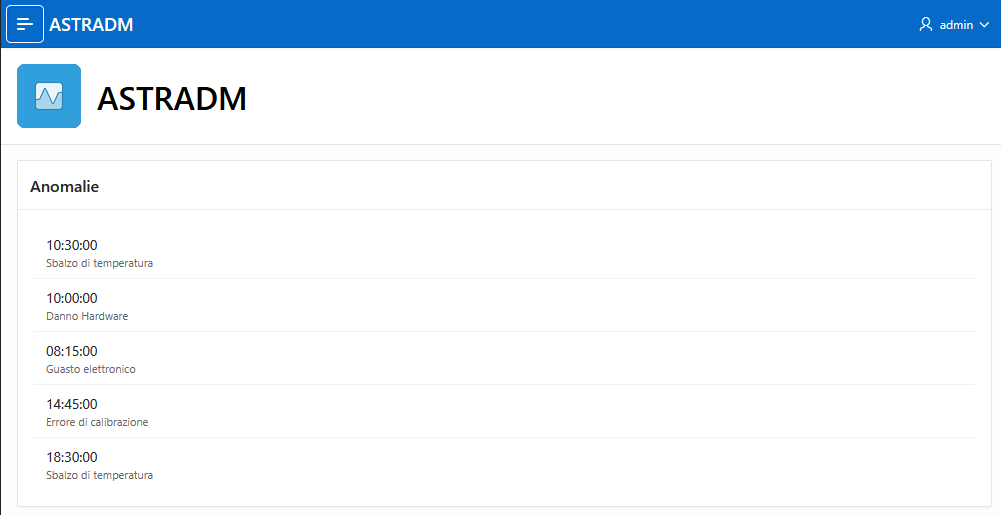
\includegraphics[width=\linewidth]{images/home-anomalie.png}
    \caption{Resoconto delle ultime 4 anomalie}
    \label{fig:anomalie}
  \end{figure}
\item Grafico a torta sullo stato dei sensori
  \begin{figure}[ht]
    \centering
    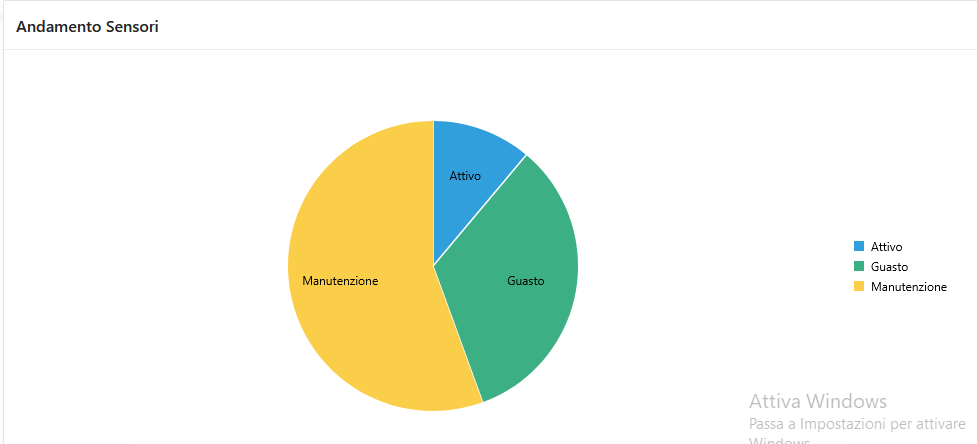
\includegraphics[width=\linewidth]{images/home-sensori.png}
    \caption{Grafico rappresentante lo stato dei sensori}
    \label{fig:sensori}
  \end{figure}
\end{itemize}
%%% Local Variables:
%%% mode: LaTeX
%%% TeX-master: "Tesina"
%%% End:

\subsubsection{Report - Missioni}
In questa pagina invece è contenuto un report in formato classico di
tutte le missioni, così da permettere un analisi più approfondita da
parte dell'operatore di tutte le missioni, completate o non.
\begin{figure}[ht]
    \centering
    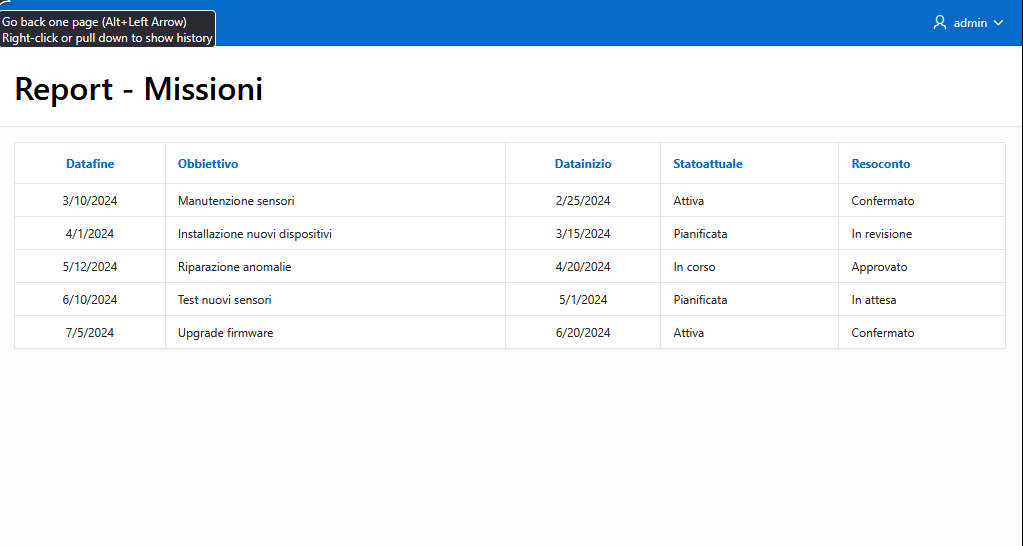
\includegraphics[width=\linewidth]{images/report-missioni.png}
    \caption{Report in formato classico di tutte le missioni}
    \label{fig:missioni}
  \end{figure}
%%% Local Variables:
%%% mode: LaTeX
%%% TeX-master: "Tesina"
%%% End:

%%% Local Variables:
%%% mode: LaTeX
%%% TeX-master: "Tesina"
%%% End:


%%% Local Variables:
%%% mode: LaTeX
%%% TeX-master: "Tesina"
%%% End:

\end{document}

%%% Local Variables:
%%% mode: LaTeX
%%% TeX-master: "Tesina"
%%% End:
